% !TEX TS-program = pdflatex
% !TEX encoding = UTF-8 Unicode

% This is a simple template for a LaTeX document using the "article" class.
% See "book", "report", "letter" for other types of document.

\documentclass[11pt]{article} % use larger type; default would be 10pt

\usepackage[utf8]{inputenc} % set input encoding (not needed with XeLaTeX)
\usepackage{german}
%%% Examples of Article customizations
% These packages are optional, depending whether you want the features they provide.
% See the LaTeX Companion or other references for full information.

%%% PAGE DIMENSIONS
\usepackage{geometry} % to change the page dimensions
\geometry{a4paper} % or letterpaper (US) or a5paper or....
% \geometry{margins=2in} % for example, change the margins to 2 inches all round
% \geometry{landscape} % set up the page for landscape
%   read geometry.pdf for detailed page layout information

\usepackage{graphicx} % support the \includegraphics command and options

% \usepackage[parfill]{parskip} % Activate to begin paragraphs with an empty line rather than an indent

%%% PACKAGES
\usepackage{booktabs} % for much better looking tables
\usepackage{array} % for better arrays (eg matrices) in maths
\usepackage{paralist} % very flexible & customisable lists (eg. enumerate/itemize, etc.)
\usepackage{verbatim} % adds environment for commenting out blocks of text & for better verbatim
\usepackage{subfig} % make it possible to include more than one captioned figure/table in a single float
\usepackage{german}
\usepackage{url}
\usepackage{hyperref}
\usepackage{amsfonts}
\usepackage{amsmath}
\usepackage{amsthm}
\usepackage{listings}
% These packages are all incorporated in the memoir class to one degree or another...

\usepackage{listings}
\usepackage{color}
\definecolor{lightgray}{rgb}{.9,.9,.9}
\definecolor{darkgray}{rgb}{.4,.4,.4}
\definecolor{purple}{rgb}{0.65, 0.12, 0.82}

\lstdefinelanguage{JavaScript}{
  keywords={typeof, new, true, false, catch, function, return, null, catch, switch, var, if, in, while, do, else, case, break},
  keywordstyle=\color{blue}\bfseries,
  ndkeywords={class, export, boolean, throw, implements, import, this},
  ndkeywordstyle=\color{darkgray}\bfseries,
  identifierstyle=\color{black},
  sensitive=false,
  comment=[l]{//},
  morecomment=[s]{/*}{*/},
  commentstyle=\color{purple}\ttfamily,
  stringstyle=\color{red}\ttfamily,
  morestring=[b]',
  morestring=[b]"
}

\lstset{
   language=JavaScript,
   backgroundcolor=\color{lightgray},
   extendedchars=true,
   basicstyle=\footnotesize\ttfamily,
   showstringspaces=false,
   showspaces=false,
   %numbers=left,
   numberstyle=\footnotesize,
   numbersep=9pt,
   tabsize=2,
   breaklines=true,
   showtabs=false,
   captionpos=b
}

%%% HEADERS & FOOTERS
\usepackage{fancyhdr} % This should be set AFTER setting up the page geometry
\pagestyle{fancy} % options: empty , plain , fancy
\renewcommand{\headrulewidth}{0pt} % customise the layout...
\lhead{}\chead{}\rhead{}
\lfoot{}\cfoot{\thepage}\rfoot{}

%%% SECTION TITLE APPEARANCE
\usepackage{sectsty}
\allsectionsfont{\sffamily\mdseries\upshape} % (See the fntguide.pdf for font help)
% (This matches ConTeXt defaults)

%%% ToC (table of contents) APPEARANCE
\usepackage[nottoc,notlof,notlot]{tocbibind} % Put the bibliography in the ToC
\usepackage[titles,subfigure]{tocloft} % Alter the style of the Table of Contents
\renewcommand{\cftsecfont}{\rmfamily\mdseries\upshape}
\renewcommand{\cftsecpagefont}{\rmfamily\mdseries\upshape} % No bold!

%%% END Article customizations

%%% The "real" document content comes below...

\theoremstyle{definition}
\newtheorem*{beisp}{Beispiel}
\newtheorem{definition}{Definition}
\newtheorem*{bemerkung}{Bemerkung}

\title{Darstellung von Differentialgleichungen mit einem zellulären Automaten}
\author{Detlev Ziereisen, Florian Lüthi, i10b}
%\date{} % Activate to display a given date or no date (if empty),
         % otherwise the current date is printed 

\begin{document}
\maketitle

\tableofcontents

\section{Einleitung}

Diese Projektarbeit (bestehend aus diesem Dokument sowie der zugehörigen Software {\tt Tusk}) hat zum Ziel, partielle Differentialgleichungen aus dem Umfeld der physikalischen Simulationen mit einem zellulären Automaten zu berechnen sowie darzustellen. Es soll gezeigt werden, dass dies unter den konzeptionellen Restriktionen der Theorie der zellulären Automaten möglich ist, insbesondere soll die Annahme Konrad Zuses, dass die Naturgesetze diskreten Regeln folgten und das gesamte Geschehen im Universum das Ergebnis der Arbeit eines gigantischen zellulären Automaten sei \cite{wiki:zellautomat, zuse1969}, zumindest für den Scope dieser Arbeit bestätigt werden. Ausserdem soll gezeigt werden, dass die intuitiv erwarteten Resultate in sinnvoller Rechenzeit dargestellt werden können.

Diese Projektarbeit wurde im Rahmen des Kurses Softwareprojekt 2 an der Hochschule für Technik Zürich durchgeführt. Der Quellcode sowie auch dieses Dokument sind Online auf \url{http://www.github.com/foyan/Tusk} zu finden.

Das vorliegende Dokument ist so gegliedert, dass im folgenden Kapitel die nötigen theoretischen Grundsteine über zelluläre Automaten, numerische Lösung von Differentialgleichungen sowie die Verknüpfung dieser beiden Aspekte gelegt werden. Daraufhin werden ausgewählte Bereiche der Implementation kommentiert, und zu guter Letzt folgt ein Résumé, das sich mit der Beantwortung oder Nichtbeantwortbarkeit der eingangs gestellten Fragen und Thesen beschäftigt.

Der Autoren Dank geht (in alphabetischer Reihenfolge der Vornamen) an Albert Heuberger für geballte mathematische Kompetenz gepaart mit unendlicher Geduld, an Lukas Eppler für die ständige Begleitung, sowie an Philippe Nahlik für die tolle Kursführung.

\part{Theorie}

\section{Zelluläre Automaten}

\begin{quote}Ein zellulärer Automat ist eine regelmäßige Annordnung von Zellen. Jede Zelle kann eine endliche Zahl
von Werten / Zuständen annehmen und hat eine begrenzte Zahl von Nachbarzellen, die sie beeinflussen
können. Das Muster des gesamten zellulären Automaten ändert sich in einzelnen Schritten, die durch eine
Reihe von Übergangsregeln bestimmt werden, die für alle Zellen gelten.\cite{beckmann}\end{quote}

Also:

\begin{definition}[Zellulärer Automat] Ein zellulärer Automat ist durch folgende Eigenschaften festgelegt:
\begin{itemize}
\item einen Zellularraum $R$,
\item eine endliche Nachbarschaft $N$, wobei $\forall r \in R \left(N_r \subset R\right)$,
\item eine Zustandsmenge $Q$,
\item eine Überführungsfunktion $\delta: Q^{|N| + 1}\mapsto Q$.
\end{itemize}
Die Zustandsübergänge erfolgen für alle Zellen nach derselben Überführungsfunktion und gleichzeitig. Die Zellzustände können wie die Zeitschritte diskret sein. \cite{wiki:zellautomat}

\end{definition}

\begin{bemerkung}
Aus dieser Definition folgt unmittelbar, dass der neue Zustand einer Zelle nur vom momentanen Zustand dieser Zelle sowie den Zuständen der Nachbarzellen abhängig sein kann.
\end{bemerkung}

Für zweidimensional organisierte $R$ sind zwei Arten von Nachbarschaft üblich:
\begin{description}
\item[Von-Neumann-Nachbarschaft] Die Nachbarschaft besteht jeweils aus den vier geographisch nächsten Nachbarzellen: $N_{i,j} = \left\{ R_{i,j-1}, R_{i,j+1}, R_{i-1,j}, R_{i+1,j}\right\}$
\item[Moore-Nachbarschaft] Die Nachbarschaft besteht jeweils aus allen Zellen der Von-Neumann-Nachbarschaft sowie zusätzlich der diagonalen Nachbarzellen:

$N_{i,j} = \left\{ R_{i,j-1}, R_{i,j+1}, R_{i-1,j}, R_{i+1,j},R_{i-1,j-1}, R_{i-1,j+1}, R_{i-1,j+1}, R_{i+1,j+1} \right\}$ \cite{schurr}
\end{description}

\begin{beisp}[Wolfram's eindimensionales Universum] Stephen Wolfram\footnote{Stephen Wolfram (* 29. August 1959), britischer Physiker und Mathematiker, Schöpfer der Software Mathematica sowie der Suchmaschine Wolfram Alpha \cite{wiki:wolfram}} definiert in \cite{wolfram2002} und in etlichen Arbeiten aus der Mitte der 1980er-Jahre einen parametrierbaren zellulären Automaten, der nur aus einer einzigen Raumdimension besteht\cite{wiki:wolfram}. In seiner einfachsten Ausprägung ist die Nachbarschaft $N_i$ definiert als $\left\{ R_{i-1}, R_{i+1} \right\}$, und jede Zelle kann genau zwei Zustände annehmen (tot und lebendig bzw. $0$ und $1$). Damit ist
\begin{equation*}
\delta : \left\{0,1\right\}^{|\left\{ R_{i-1}, R_{i+1}\right\}|+ 1} \mapsto \left\{0,1\right\} = \left\{0,1\right\}^3 \mapsto \left\{0,1\right\},
\end{equation*}
ergo existieren 8 mögliche Zustandsänderungen. Ein Beispiel:

\begin{table}[here]
\begin{center}
\begin{tabular}{|r||c|c|c|c|c|c|c|c|}
\hline
alte $R_{i-1}R_iR_{i+1}$ &111& 110 & 101 &100 &011 &010 &001 &000  \\\hline
neues $R_i$ & 0 & 1 & 1 & 0& 1 & 1 & 1 & 0 \\\hline
\end{tabular}
\end{center}
\caption{Wolfram-Konfiguration 110}
\label{wolfram110}
\end{table}

Man stellt nun fest, dass bei 8 möglichen Zustandsänderungen für die Anzahl der möglichen Konfigurationen gilt:
\begin{equation*}
|K| = |Q|^{|\operatorname{dom}(\delta)|} = 2^8 = 256.
\end{equation*}
Jeder dieser Konfigurationen kann eine natürliche Zahl $\left\{0, 1, 2, \dots, 255\right\}$ zugeordnet werden, indem die neuen $R_i$ wie oben tabelliert und pro Zeile als binäre Zahl aufgefasst werden \cite{betz2003}:

\begin{table}[here]
\begin{center}
\begin{tabular}{|c|c|c|c|c|c|c|c||l|}
\hline
111 & 110 & 101 &100 &011 &010 &001 &000 & Zahl \\\hline\hline
 0 & 0 & 0 & 0& 0 & 0 & 0 & 0 & $00000000_b = 0_d$ \\\hline
 0 & 0 & 0 & 0& 0 & 0 & 0 & 1 & $00000001_b = 1_d$ \\\hline
 0 & 0 & 0 & 0& 0 & 0 & 1 & 0 & $00000010_b = 2_d$ \\\hline
\multicolumn{9}{|c|}{$\vdots$} \\\hline
 0 & 1 & 1 & 0& 1 & 1 & 1 & 0 & $01101110_b = 110_d$ \\\hline
\multicolumn{9}{|c|}{$\vdots$} \\\hline
 1 & 1 & 1 & 1& 1 & 1 & 1 & 1 & $11111111_b = 255_d$ \\\hline
\end{tabular}
\end{center}
\caption{Alle Wolfram-Konfigurationen}
\label{wolframalle}
\end{table}

Dadurch ist es möglich, sämtliche eindimensionalen Wolfram-Universen durch eine einzige Zahl zu identifizieren.

Als besonders spannend hat sich die in Tabelle \ref{wolfram110} dargestellte Konfiguration 110 erwiesen, weil sie die Eigenschaft hat, ein Turing-vollständiges System zu sein \cite{betz2003, wolfram2002}. Dadurch ist sie die Konfiguration einer universellen Turingmaschine, die mit nur 2 Zuständen und 5 Symbolen umgesetzt werden kann -- somit hat die Wolfram-Konfiguration 110 als Turingmaschine einen Umfang von $2\cdot 5 = 10$ und zählt damit zu den kleinsten bis dato bekannten Turingmaschinen \cite{betz2003}.

\end{beisp}

\begin{beisp}[Game of Life]

\newcommand{\ql}{q_\textrm{lebend}}
\newcommand{\qt}{q_\textrm{tot}}

Das von Conway\footnote{John Horton Conway (* 26. Dezember 1937), englischer Mathematiker\cite{wiki:conway}} 1970 entworfene Game of Life ist eine bis heute populäre Umsetzung der Automatentheorie und insbesondere der Idee der zellulären Automaten \cite{wiki:gameoflife}.

Der ursprüngliche Entwurf befindet sich in einem zweidimensionalen $R$ unter Verwendung der Moore-Nachbarschaft. Die Zellen können zwei mögliche Zustände $\left\{\ql, \qt \right\}$ annehmen, und die Übergangsfunktion ist definiert \cite{Hafner} als:
\begin{equation*}
\delta(r, N) = \begin{cases}
\ql & (r = \qt \land \varsigma(\ql,N) = 3) \\
\qt & (r = \ql \land \varsigma(\ql, N) < 2) \\
\ql & (r = \ql \land 2 \leq \varsigma(\ql, N) \leq 3) \\
\qt & (r = \ql \land  \varsigma(\ql, N) > 3) \\
\qt & (\textrm{sonst})
\end{cases}
\end{equation*}
unter Zuhilfenahme der Statuszählfunktion
\begin{equation*}
\varsigma(q, N) = \sum\limits_{i=1}^8  \begin{cases} 1 & (N_i = q) \\ 0 & (N_i \neq q) \end{cases}
\end{equation*}

\end{beisp}

\section{Vom zellulären Automaten zur Differentialgleichung}

Die Berechnung und Darstellung physikalischer Begebenheiten (allgemein ausgedrückt durch folgende partielle Differentialgleichung, mit $u: u(\vec{x}, t)$)
\begin{equation*}
k_n \frac{\partial^n u}{\partial t^n} + k_{n-1} \frac{\partial^{n-1} u}{\partial t^{n-1}} + \cdots + k_1 \frac{\partial u}{\partial t} + k_0 = \frac{\partial^n u}{\partial  \vec{x}^n} + \frac{\partial^{n-1}}{\partial \vec{x}^{n-1}} + \cdots + \frac{\partial u}{\partial \vec{x}}
\end{equation*}
mit zellulären Automaten kann durchgeführt werden, indem folgendes getan wird:
\begin{itemize}
\item $R$ entspricht einer sinnvollen (groben) Diskretisierung der örtlichen Variablen $\vec{x}$ in einer, zwei oder drei Dimensionen
\item Jede Zelle in $R$ ist ein Tupel $(Q, D)$ mit $Q$ als einer Menge von berechnungsfernen Zustandsinformationen und den Differentialen nach der Zeit
\[
D = \left( u, \frac{\partial u}{t}, \frac{\partial^2 u}{\partial t^2}, \cdots, \frac{\partial^n u}{t^n} \right)  \in \mathbb{R}^n
\]
\item Eine neue Generation entspricht jeweils der fortgelaufenen Zeit $\partial t$, welche sehr fein diskretisiert werden muss
\item In der Übergangsfunktion $\delta$ steckt die eigentliche Differentialgleichung. In der Regel verändert sie nur die Elemente von $D$. Sollte die Differentialgleichung Terme mit verschiedenen Ordnungen enthalten, wird die Gleichung unter Zuhilfenahme entsprechender Hilfsgleichungen $\lambda_1, \lambda_2, \dots, \lambda_n$ in ein äquivalentes System gewöhnlicher Differentialgleichungen umgeformt. 
\end{itemize}

\section{Numerische Lösung von Differentialgleichungen}

Damit die numerische Lösung von Differentialgleichungen gelingt, sind vor allem zwei Fertigkeiten vonnöten: Die numerische Differenzierung sowie die numerische Integration. Wir wollen beide Gebiete kurz streifen, und zwar unter den für uns nützlichen Gesichtspunkten bezüglich der Wahl der Variablen sowie der vorliegenden impliziten Funktionen (beziehungsweise diskreten Werten als Zellinhalte des zellulären Automaten).

\subsection{Differenzierung nach dem Ort}

%Wir starten mit der homogenen Wellengleichung
%\begin{equation*}
%\frac{\partial^2 u}{\partial t^2} = k\cdot \frac{\partial^2 u}{\partial \vec{x}^2}
%\end{equation*}

Wir starten mit den gegebenen Werten $u_{\vec x}$ (den Zuständen der Zellen aus $R$). Daraus erhalten wir die diskrete Funktion
\[
u: R \mapsto \mathbb{R}, u(\vec x) = u_{\vec x}
\]

welche durch komponentenweises Einsetzen des Differenzenquotienten $\frac {\Delta u}{\Delta \vec x}$ folgendermassen differenzierbar ist (unter Zuhilfenahme des Einheitsvektors $\vec e_i$ für jede Komponente von $\vec x$ sowie der Erkenntnis, dass durch die diskrete Ausgangsfunktion $\Delta \vec{x}$ komponentenweise $1$ ist; die Interpretation, wo genau sich die Nachbarzelle $\vec x \pm n\cdot\vec e$ befindet, überlassen wir der für den zellulären Automaten gültigen Nachbarschaftsfunktion):
\begin{equation}\label{diffone}
	\left(\frac {\Delta}{\Delta \vec x} u\right)_{\vec x} = u_{\vec x} - \sum\limits_{i=1}^{\dim(\vec x)} u_{\vec x - \vec e_i}
\end{equation}
Diese Differenzen können natürlich wiederum differenziert werden:
\begin{eqnarray*}
	\left(\frac{\Delta}{\Delta \vec x}\left( \frac {\Delta}{\Delta \vec x} u \right)_{\vec x}\right)_{\vec x} &=& \left(\frac {\Delta}{\Delta \vec x} u\right)_{\vec x} - \sum\limits_{i=1}^{\dim(\vec x)} \left( \frac {\Delta}{\Delta \vec x} u \right)_{\vec x - \vec e_i}
\end{eqnarray*}
Durch Einsetzen von \ref{diffone} in die obige Gleichung ergibt sich dann für die Differenz zweiter Ordnung:
\begin{eqnarray*}
\left( \frac{\Delta^2}{\Delta \vec x^2} u\right)_{\vec x} &=& u_{\vec x} - \sum\limits_{i=1}^{\dim(\vec x)} u_{\vec x - \vec e_i} - 
\sum\limits_{i=1}^{\dim(\vec x)} \left( u_{\vec {x^*}} - \sum\limits_{i=1}^{\dim(\vec x)} u_{\vec {x^*} - \vec e_i} \right)_{\vec {x^*} := \vec x - \vec e_i} \\
&=& u_{\vec x} - \sum\limits_{i=1}^{\dim(\vec x)} u_{\vec x - \vec e_i} - \sum\limits_{i=1}^{\dim(\vec x)} u_{\vec x - \vec e_i} + \sum\limits_{i=1}^{\dim(\vec x)} u_{\vec x - 2\vec e_i} \\
&=&  u_{\vec x} - 2\cdot\sum\limits_{i=1}^{\dim(\vec x)} u_{\vec x - \vec e_i} + \sum\limits_{i=1}^{\dim(\vec x)} u_{\vec x - 2\vec e_i}
\end{eqnarray*}

\begin{bemerkung}[Indizes]
Da der Definitionsbereich der besprochenen Funktion diskret ist, verringert sich die Kardinalität des Definitionsbereichs der Differenzen mit fortschreitender Ordnung jeweils um $1$ pro Dimension. Geographisch gesprochen, liegt die Differenz zweier Zellen ja eigentlich auf der gemeinsamen Kante dieser zwei Zellen. Daher ist es in der Praxis sinnvoll, die Differenzen gerader Ordnungen (bei deren Berechnung wie eben gesehen 3 Zellen pro Dimension involviert sind) jeweils in die Zelle in der Mitte zu schieben. Im Falle der zweiten Ordnung ergibt sich damit:
\begin{equation}
\left( \frac{\Delta^2}{\Delta \vec x^2} u\right)_{\vec x} =\sum\limits_{i=1}^{\dim(\vec x)} u_{\vec x - \vec e_i}  -2\cdot u_{\vec x} + \sum\limits_{i=1}^{\dim(\vec x)} u_{\vec x + \vec e_i}
\end{equation}
\end{bemerkung}

\subsection{Integration nach der Zeit mit Einschrittverfahren}

\newcommand{\intr}{\mathbf{int}}
\renewcommand{\d}{\mathrm{d}}
\newcommand{\duxt}{\left(\frac{\Delta}{\Delta \vec x}u \right)_{\vec x, t}}
\newcommand{\duxtp}[1]{\left(\frac{\Delta}{\Delta \vec x}u \right)_{\vec x, t + #1 h}}

\subsubsection{Forderung}

Wir starten mit den gegebenen Werten $\left(\frac{\Delta}{\Delta \vec x}u \right)_{\vec x}$ (den vorgängig berechneten Differenzen zwischen den Zellen). Wir definieren die allgemeine Integrationsfunktion
\[
\intr :  \mathbb{R}^2 \mapsto \mathbb{R}
\]
für welche jeweils gelten muss:
\[
\intr\left(\duxt, h \right) \approx \int\limits_t^{t+h} u_{\vec x} \d t
\]

Da die $u_{\vec x}$ zu jedem Zeitpunkt $t$ (also pro Zeitschritt $h$ beziehungsweise $\d t$) jeweils von ihren Nachbarzellen abhängen, ist es vonnöten, sämtliche Zellen für einen einzigen Zeitschritt simultan durchzurechnen.

\subsubsection{Die impliziten Runge-Kutta-Verfahren}

Da uns hier nur Einschrittverfahren interessieren, schauen wir uns im Detail die Klasse der Runge-Kutta-Verfahren\footnote{Carl David Tolmé Runge (1856--1927), deutscher Mathematiker \cite{wiki:Runge}}\footnote{Martin Wilhelm Kutta (1867--1944), deutscher Mathematiker \cite{wiki:Kutta}} an, welche auf dem expliziten Euler-Verfahren\footnote{Leonhard Euler (1707--1783), Schweizer Mathematiker und Physiker \cite{wiki:Euler}} basieren und durch Butcher-Tableaux\footnote{John Charles Butcher (*1933), neuseeländischer Mathematiker \cite{wiki:Butcher}} allgemein definiert werden können.

Sämtliche Runge-Kutta-Verfahren können folgendermassen dargestellt werden:
\[
y_{n+1} = y_n + h\cdot \sum\limits_{j=1}^s \gamma_j \cdot k_j
\]
wobei $h$ die gewählte Schrittweite, $\gamma_j$ die charakteristischen Koeffizienten des gewählten Verfahrens sowie $k_j$ die Auswertungen der zu integrierenden Funktion $f$ an bestimmten Stützstellen repräsentieren. Für $k_j$ gilt dann:
\[
k_j = f\left(t_n + h\cdot\alpha_j, y^n + h\cdot \sum\limits_{i=1}^m \beta_{j,i}\cdot k_i \right)
\]

wobei $\alpha_j$ sowie $\beta_{j,i}$ wiederum charakteristische Koeffizienten sind \cite{Massjung, wiki:RungeKutta}, welche zusammen mit den $\gamma_j$ in einem Butcher-Tableau folgendermassen angeordnet werden können:
\[
\begin{bmatrix}
\begin{array}{c|c}
a & B\\
\hline     & c \\
\end{array}
\end{bmatrix} = \begin{bmatrix}
\begin{array}{c|cccc}
  \alpha_1    & \beta_{1,1} & \beta_{1,2}& \cdots & \beta_{1,m}\\
  \alpha_2    & \beta_{2,1} & \beta_{2,2}& \cdots & \beta_{2,m}\\
  \vdots & \vdots & \vdots& \ddots& \vdots\\
  \alpha_m    & \beta_{m,1} & \beta_{m,2}& \cdots & \beta_{m,m}\\
  \hline & \gamma_1    & \gamma_2   & \cdots & \gamma_m\\
\end{array}

\end{bmatrix}
\]

Runge-Kutta-Verfahren sind im Allgemeinen implizit, weil zur Bestimmung der $k_j$ sowie $y^{n+1}$ ein (mindestens lineares) $(m+1)\times(m+1)$-Gleichungssystem gelöst werden muss; dies verursacht natürlich entsprechende Kalamitäten. Solchartige Verfahren sind aber sehr stabil.\cite{Deuflhard}

\subsubsection{Die expliziten Runge-Kutta-Verfahren}

Ist es nun möglich, Koeffizienten zu finden, deren Matrix $B$ strikte nilpotente untere Dreiecksgestalt hat, so spricht man von einem expliziten Verfahren, weil sich das Gleichungssystem einfach durch Rückwärtseinsetzen lösen lässt (sogar wenn es nichtlinear ist):

\[
\begin{bmatrix}
\begin{array}{c|c}
a & B\\
\hline     & c \\
\end{array}
\end{bmatrix} = \begin{bmatrix}
\begin{array}{c|cccc}
  \alpha_1 & 0  \\
  \alpha_2    & \beta_{2,1} & 0\\
  \vdots & \vdots & \vdots& \ddots\\
  \alpha_m    & \beta_{m,1} & \beta_{m,2}& \cdots & 0\\
  \hline & \gamma_1    & \gamma_2   & \cdots & \gamma_m\\
\end{array}

\end{bmatrix}
\]

Für ausgewählte explizite Verfahren lassen sich nun sowohl Butcher-Tableau als auch die geforderte Integrationsfunktion $\intr$ folgendermassen aufstellen:

\begin{description}
\item[Euler]
\begin{eqnarray*}
\begin{bmatrix}
\begin{array}{c|c}
a & B\\
\hline     & c \\
\end{array}
\end{bmatrix}
 &=& \begin{bmatrix}
\begin{array}{c|c}
0 & 0 \\\hline
& 1
\end{array}
\end{bmatrix} \\
\Rightarrow \intr\left(\duxt, h\right) &=& u_{\vec x, t} + h\cdot \duxt
\end{eqnarray*}

\item[Runge-Kutta 2. Ordnung]
\begin{eqnarray*}
\begin{bmatrix}
\begin{array}{c|c}
a & B\\
\hline     & c \\
\end{array}
\end{bmatrix} &=& \begin{bmatrix}
\begin{array}{c|cc}
0 & 0 \\
\frac 1 2 & \frac 1 2 & 0 \\\hline
& 0 & 1
\end{array}
\end{bmatrix} \\
\Rightarrow \intr\left(\duxt, h\right) &=& u_{\vec x, t} + h\cdot k_2 \\
%k_2 &=& \left(\frac{\Delta}{\Delta t} u \right)_{\vec x, t + \frac 1 2 h} \\
%&=&  u_{\vec x, t} + h\cdot\intr\left(\duxtp{\frac 1 2} \right) \\
&=&  u_{\vec x, t} + h\cdot\intr\left(\duxtp{\frac 1 2} \right) \\
\end{eqnarray*}

\item[Runge-Kutta 4. Ordnung]
\[
\begin{bmatrix}
\begin{array}{c|c}
a & B\\
\hline     & c \\
\end{array}
\end{bmatrix} = \begin{bmatrix}
\begin{array}{c|cccc}
0 & 0 \\
\frac 1 2 & \frac 1 2 & 0 \\
\frac 1 2 & 0 & \frac 1 2 & 0 \\
1 & 0 & 0 & 1 & 0 \\\hline
& \frac 1 6 & \frac 1 3 & \frac 1 3 & \frac 1 6
\end{array}
\end{bmatrix}
\]
\end{description}

\subsection{Die homogene Wellengleichung}

Am Beispiel der homogenen Wellengleichung soll nun die Umsetzung einer Differentialgleichung in einem zellulären Automaten gezeigt werden. Die homogene Wellengleichung ist eine partielle Differentialgleichung zweiter Ordnung und lautet \cite{wiki:Wellengleichung}:
\[
\frac 1 {c^2} \frac{\partial^2 u}{\partial t^2}-\sum_{i=1}^{n} \left( \frac{\partial^2 u}{\partial x_i^2} \right)  = 0
\]

oder ein bisschen umgeformt ($\frac 1 {c^2} = \frac 1 k$) und die Einzelkomponenten $x_1, x_2, \dots, x_n$ als Vektor geschrieben:
\[
\frac {\partial^2 u} {\partial \vec x^2} = k \cdot \frac {\partial^2 u}{\partial t^2}
\]

Nach diesem Schema soll zweimal nach dem Ort differenziert und zweimal nach der Zeit integriert werden:

%\begin{equation*}
%\begin{array}{rcl}
\begin{align*}
u_i &&& u_i(t+\Delta t) = u_i(t) +  \frac{\partial u_i(t+\Delta t)}{\partial t}\Delta t \\
\downarrow &&& \uparrow \\
\frac{\partial u_i}{\partial \vec x} = u_i - \sum u_{i-1} &&& \frac{\partial u_i(t+\Delta t)}{\partial t} = \frac{\partial u_i(t)}{\partial t} + \frac{\partial^2 u}{\partial t^2}\Delta t \\
\downarrow &&& \uparrow \\
\frac{\partial^2 u_i}{\partial \vec x^2} = -2u_i + \sum u_{i-1} + \sum u_{i+1} & \underbrace{\longrightarrow}_{\frac{\partial^2 u}{\partial t^2} = k\cdot \frac{\partial^2 u}{\partial \vec{x}^2}} && \frac{\partial^2 u}{\partial t^2}
\end{align*}
%\end{array}
%\end{equation*}

Als Nachbarschaft wird die Von-Neumann-Nachbarschaft gewählt, weil bei der Moore-Nachbarschaft die Eckzellen nicht linear unabhängig wären. Ergo ergibt sich folgende Übergangsfunktion $\delta$, abhängig von der Zelle $r$ sowie den Nachbarzellen $n, e, s, w$ (Norden, Osten, Süden, Westen für ein zweidimensionales Zellfeld):

\begin{eqnarray*}
\delta(r, n, e, s, w) &=& \begin{bmatrix}
	\delta_{\frac {\Delta r}{\Delta t}}(r,n,e,s,w) \\
	\delta_{\frac {\Delta^2 r}{\Delta t^2}}(r,n,e,s,w)
\end{bmatrix} \\
&=& \begin{bmatrix}
	r_{\frac {\Delta r}{\Delta t}} + \delta_{\frac {\Delta^2 r}{\Delta t^2}}(r,n,e,s,w)  \cdot \Delta t \\
	\frac{\Delta^2 r}{\Delta \vec x^2} \cdot k  \\
\end{bmatrix} \\
&=& \begin{bmatrix}
	r_{\frac {\Delta r}{\Delta t}} + \delta_{\frac {\Delta^2 r}{\Delta t^2}}(r,n,e,s,w)  \cdot \Delta t \\
	(-2 r + \frac 1 2 (n + e + s + w)) \cdot k
\end{bmatrix}
\end{eqnarray*}

sowie unter der Annahme, dass die Richtung der Nachbarzellen bekannt sind (d.h. jeweils der Vorgänger beziehungsweise der Nachfolger innerhalb einer Dimension bekannt sind und deswegen $N$ auch ausgedrückt werden kann als:)
\[
N^* =\begin{pmatrix} \overbrace{n_{1,1} \in N}^{\textrm{1. Dimension}} & \overbrace{n_{2,1} \in N}^{\textrm{2. Dimension}} & \cdots & \overbrace{n_{\frac{1}{2}|N|, 1} \in N}^{\textrm{$\frac{1}{2}|N|$te Dimension}} & \textrm{Vorgänger} \\
n_{1,2} \in N & n_{2,2} \in N & \cdots & n_{\frac{1}{2}|N|, 2} \in N & \textrm{Nachfolger}
 \end{pmatrix}
\]

kann die Übergangsfunktion $\delta$ für die Wellengleichung folgendermassen formuliert werden:

\begin{eqnarray*}
\delta(r, N^*) = 
\end{eqnarray*}

\part{Bemerkungen zur Implementation}

\section{Wahl des Umfelds}

Die Wahl des Umfelds fiel auf eine Kombination aus JavaScript und dem HTML5-{\tt canvas}-Element für die grafische Ausgabe. Die hauptsächlichen Gründe dafür sind die einfache Umsetzung sowie die sehr gute Portabilität, vorallem auch auf portable Devices mit Touch-Bedienung. Dadurch kommt der primäre Use Case der Software (Bewegung einer Flüssigkeit mittels dem Pointing Input) besonders gut zur Geltung, weil der Input eben mit dem Finger vorgenommen werden kann.

Bedenken wurden vorgängig und während der ersten Implementierungsphase vor allem in Bezug auf die Perfomance geäussert, konnten aber im Laufe des Projekts zerstreut werden, auch weil gezeigt werden konnte, dass Optimierungen möglich sind (paralleles Berechnen, Umstellung von Vektorgrafik-Operationen auf Bitmap-Manipulationen).

Als Alternativen waren das Game-Framework XNA sowie die 3D-LED-Installation in der Haupthalle des Zürcher Hauptbahnhofs in Betracht gezogen worden.

\section{Architektur}

Eine Übersicht über die grobe Architektur sei hier als Package-Diagramm skizziert:

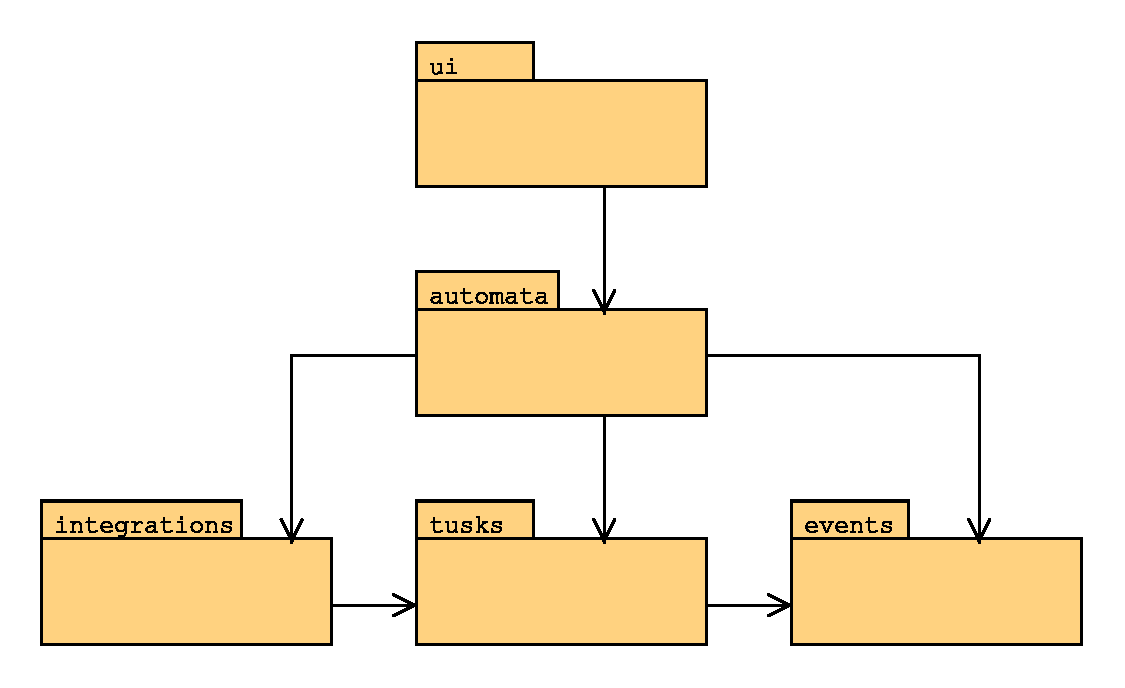
\includegraphics[scale=0.7]{uml/Architektur.pdf}

\section{Testing}

Unit Testing mit JavaScript ist nicht ganz einfach -- aber möglich und natürlich sinnvoll. Wenn die Unit Tests in einem tatsächlichen Browser auszuführen sind, weil sie beispielsweise mit dem Document Object Model interagieren, führt das zwangsläufig zu Mühsamitäten, vor allem bezüglich Continuous Integration.

Da allerdings das UI nur einen kleinen Teil unseres Programms ausmacht, schien es ratsam, vor allem die anderen Bereiche zu testen. Daraus ergibt sich die Möglichkeit, auf eine Implementation von JavaScript in einem nicht-interaktiven Kontext zu setzen. Die Wahl fiel auf Node.js, eine auf WebKit aufbauende Server-Implementation von JavaScript \cite{Node}, sowie das Test-Framework Mocha \cite{Mocha}.
Da das produktive Programm eine reine Browser-Geschichte ist, stehen während des produktiven Betriebs weder Build-Tools noch Server zur Verfügung, alle JavaScript-Files werden vom verwendenden HTML-Dokument über profane {\tt <script>}-Tags eingebunden.
Um das sich daraus ergebende Dilemma zwischen Test- und Produktionsumgebung zu lösen, werden die Komponenten über Node-Module wo nötig zusammengestöpselt, aber nur dann, wenn Node tatsächlich zur Verfügung steht (der Ausführer also ein Test Runner ist):

\begin{lstlisting}
if (typeof(module) != "undefined") {
	module.exports = CellularAutomata;
	var Cell = require('../../src/automata/Cell.js');
	var Swimmer = require('../../src/automata/Swimmer.js');
}
\end{lstlisting}

Ein Unit Test (unter Verwendung der Should-Assertion Library) sieht dann beispielsweise folgendermassen aus:

\begin{lstlisting}
describe('CellularAutomata', function() {

	it('should step without Tusk', function() {
		var auto = new CellularAutomata();
		auto.initCells();
		var iterations = auto.iterations;
		auto.step();
		auto.iterations.should.equal(iterations+1);
	});

});
\end{lstlisting}

Die Summe der Tests kann dann auf der Kommandozeile (oder durch einen CI-Server) aufgerufen werden mit:
\begin{verbatim}
~/node node_modules/mocha/bin/mocha
\end{verbatim}

\section{Automata}

Die Klasse {\tt CellularAutomata} implementiert zusammen mit ihren Hilfsklassen den zellulären Automaten:

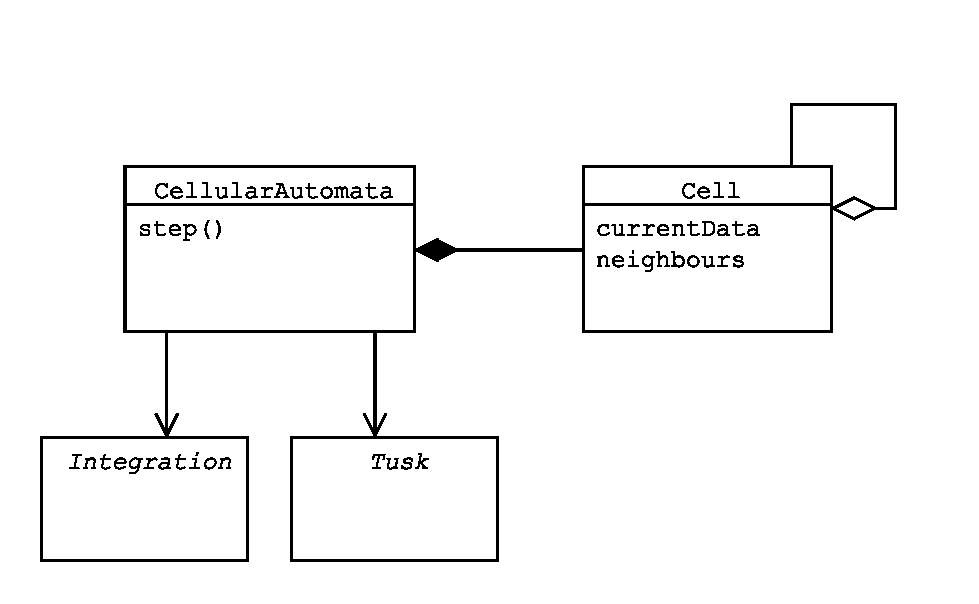
\includegraphics[scale=0.7]{uml/Automata.pdf}

{\tt CellularAutomata} definiert zuallererst einmal eine coole Hilfsmethode, welche über alle Zellen des Automaten iteriert und eine beliebige Funktion ausführt:

\begin{lstlisting}
this.forEachCell = function(fn) {
	for (var x = 0; x < this.cols; x++) {
		for (var y = 0; y < this.rows; y++) {
			var cell = this.model[x][y];
			fn(cell);
		}
	}
};
\end{lstlisting}

Diese Methode wird dann beispielsweise während der Initialisierung der Zellen folgendermassen verwendet\footnote{Ein Wort zu der auf den ersten Blick unnötig komplizierten Definition der von {\tt this.forEachCell()} auszuführenden anonymen Funktion: In JavaScript wird der Scope von Variablen durch die Funktion und nicht den Block begrenzt, darum gilt als Best Practice zur expliziten Scope-Gebung im Allgemeinen das Wrappen in einer anonymen Funktion und unmittelbarer Ausführung derselben \cite{UnderstandingClosures}. Da {\tt this} schlussendlich auch nur eine Variable in einem Funktionsscope ist, wäre {\tt this.tusk} keine sinnvolle Referenz, weil {\tt this} nicht bedingungslos (wie in anderen funktionalen Programmiersprachen üblich) eine Instanz von {\tt CellularAutomata} (den Definitionsscope von {\tt wireNeighbourCells()}), sondern der Caller ist (falls das Drücken eines Buttons zu einem Aufruf von {\tt wireNeighbourCells()} führte, wäre {\tt this} das Browser-{\tt document}).}:
\begin{lstlisting}
this.wireNeighbourCells = function() {
	if (this.tusk != null) {
		this.forEachCell(
			(function(automata) {
				return function(cell) {
					cell.neighbours = automata.tusk.getNeighbours(cell, automata.model);
				};
			})(this)
		);
	}
}
\end{lstlisting}

Des weiteren führt {\tt CellularAutomata} die Zelltransitionen durch:

\begin{lstlisting}
this.step = function() {		
	if (this.tusk != null) {
		this.fireEvents();		
		this.integration.integrate(this);
		this.travelSwimmers();
	}	
	this.iterations++;	
}
\end{lstlisting}

Spannend hierbei zu sehen ist die Aufteilung der Verantwortlichkeiten. {\tt CellularAutomata} kennt weder  die Übergangsfunktion $\delta$, die Nachbarschaftsfunktion\footnote{Wie im Listing weiter oben ersichtlich, werden sämtliche Nachbarzellen sämtlicher Zellen während der Initialisierung aufgefunden und verknüpft. Da sich gemäss der Definition des Zellulären Automaten die Nachbarschaftsbeziehungen zwischen Zellen nie ändern, ergo von Anfang an feststehen, ist dies eine zulässige Performance-Optimierung; ansonsten müsste auf das Feld der Zellen bei jedem Iterationsschritt mindestens $|R|\cdot |N|$ mal zugegriffen werden (wobei $R$ der ganze Zellraum und $N$ die Menge der Nachbarzellen einer Zelle ist).} noch die Integrationsfunktion $\intr$, sondern verwendet via Strategy-Pattern die ihr zugeteilten Implementationen (beispielsweise die Wellengleichung mit dem Euler-Verfahren).

Es ist sogar so, dass der eigentliche Zellinhalt (der ja nur von der Übergangsfunktion $\delta$ verwendet wird) unbekannt ist. Jeder Tusk besitzt entsprechend eine Factory-Methode, um einen solchen Zellinhalt herzustellen. Die Unterschiede in den Datenstrukturen sind frappant. Das Game Of Life begnügt sich mit:

\begin{lstlisting}
this.createCellData = function() {
	return {status: 0};
}
\end{lstlisting}

wogegen die Wellengleichung einige Daten mehr benötigt:
\begin{lstlisting}
this.createCellData = function() {
	return {
		u: 0,
		udx: 0,
		udxdx: 0,
		udtdt: 0,
		udt: 0,
		vx: 0,
		vy: 0
	};
};
\end{lstlisting}

\section{Integration}

Die Wahl der Integrationsmethode ist wiederum eine Anwendung des Strategy-Patterns, wie in der Übersicht skizziert:

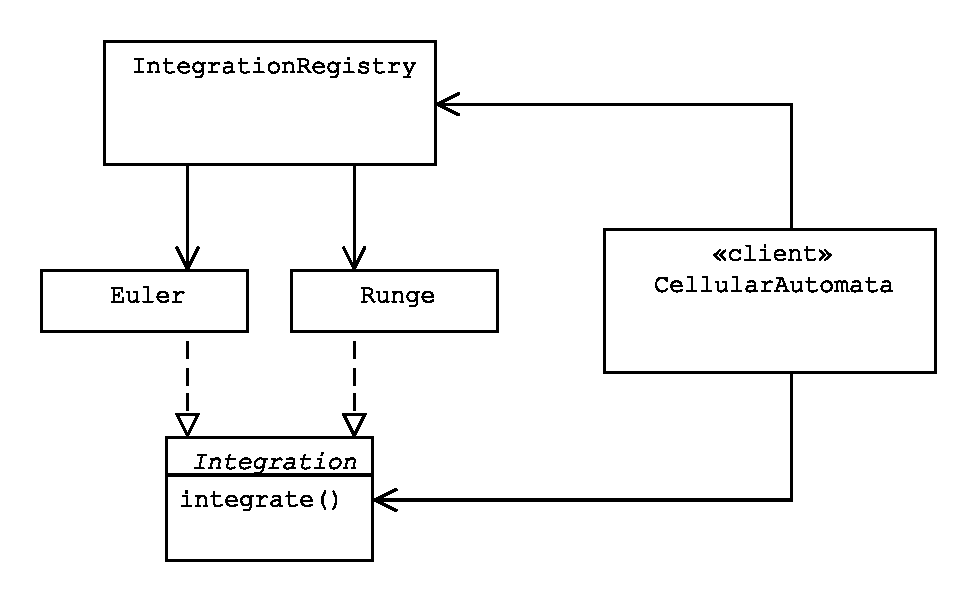
\includegraphics[scale=0.7]{uml/Integration.pdf}

{\tt integrate()} iteriert dann typischerweise über alle Zellen des Automaten und führt die Integration unter ein- oder mehrmaligem Aufruf der Übergangsfunktion $\delta$ des Tusk durch. Hier ist das Beispiel für das explizite Euler-Verfahren dargestellt:

\begin{lstlisting}
this.integrate = function(automata) {
	var dt = 1 / automata.tusk.slices;
	for (var t = 0; t < automata.tusk.slices; t++) {
		
		automata.forEachCell(
			function(cell) {
				var differentials = automata.tusk.calcDifferentials(cell, dt, function(cell2) {
					return cell2.currentData;
				});
				cell.nextData = automata.tusk.applyDifferentials(cell, dt, differentials, function(cell2) {
					return cell2.currentData;
				})
			}
		);
		
		automata.forEachCell(
			function(cell) {
				cell.currentData = cell.nextData;
			}
		);
		
	}
}
\end{lstlisting}

\section{Tusk}

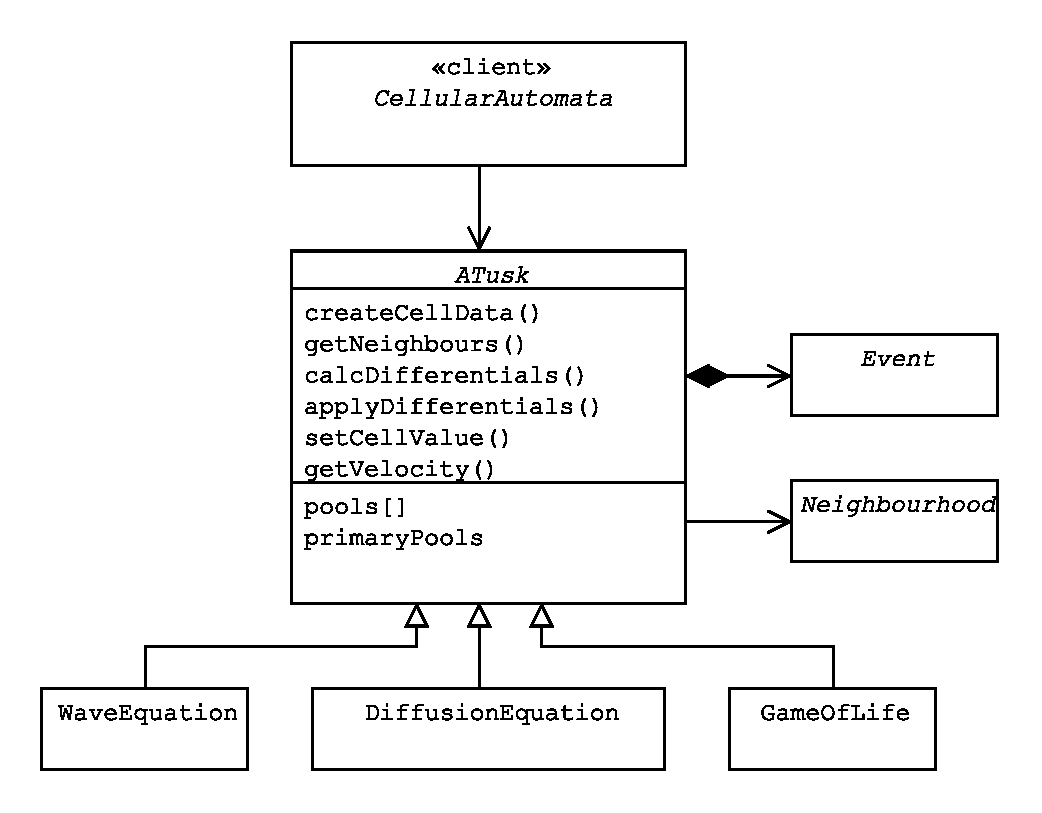
\includegraphics[scale=0.7]{uml/Tusk.pdf}

\section{Grafische Ausgabe}

Die grafische Ausgabe des zellulären Automaten findet in einem {\tt canvas}-Element statt, in das mittels JavaScript-Code gezeichnet wird. Die dafür zuständigen Klassen heissen {\tt ...CanvasPainter}, wovon verschiedene Implementationen verfügbar sind. Es wird davon ausgegangen, dass jeder {\tt ...CanvasPainter} folgende Methoden anbietet:

\begin{description}
\item[\tt begin()] Beginnt den Zeichnungszyklus.
\item[\tt updateCellView(cell)] Zeichnet eine einzelne Zelle ({\tt cell}) neu.
\item[\tt drawDuck(duck, cell)] Zeichnet eine Ente ({\tt duck}) in eine einzelne Zelle ({\tt cell}).
\item[\tt end()] Beendet den Zeichnungszyklus.
\end{description}

Die Methoden {\tt begin()} und {\tt end()} sind für Implementationen gedacht, die sich nur sinnvoll verhalten wenn sie den gesamten {\tt canvas} neu bezeichnen können und deswegen nach einem atomaren Aufruf von {\tt updateCellView()} einen inkonsistenten Zustand aufweisen.

In den folgenden Abschnitten sind die verfügbaren Implementationen grob erklärt. Es existiert ausserdem eine {\tt Noop}-Implementation, die aber trivial ist und verwendet werden kann, um die grafische Ausgabe komplett abzuschalten.

\subsection{{\tt VectorCanvasPainter}}

Diese Klasse bezeichnet den {\tt canvas} durch Vektorgrafik-Operationen:

\begin{lstlisting}
this.updateCellView = function(cell) {
	var du = cell.currentGradients; // get values
	var x = cell.x * scaleWidth; // calculate x position in pixels
	var y = cell.y * scaleHeight; //  calculate y position in pixels
	var baseColor = this.getBaseColor(); // get base painter color
	// let Tusk calculate actual cell color, and format it as 'rgb(r,g,b)'
	var color = getFormattedColor(du[this.getUIndex()], baseColor.r, baseColor.g, baseColor.b);
	this.context.fillStyle = color;
	// draw and fill a rectangle.
	this.context.fillRect(x, y, scaleWidth, scaleHeight);
};
\end{lstlisting}

\subsection{{\tt PixelCanvasPainter}}

Diese Klasse bezeichnet den {\tt canvas} durch direkte Pixel-Manipulationen. Grundsätzlich funktionert das folgendermassen \cite{mdn:PixelCanvasDoku}:

\begin{lstlisting}
var myImageData = context.createImageData(cssWidth, cssHeight);
// ... do manipulation here ...
context.putImageData(myImageData, 0, 0);
\end{lstlisting}

Es muss allerdings gesagt werden, dass die Methode {\tt putImageData()} in allen verfügbaren Implementationen (Gecko, WebKit usw.) einigermassen langsam ist. Dies wird vor allem damit erklärt, dass das zu manipulierende Pixel-Array ({\tt myImageData.data} in unserem Beispiel) ein Array von Integern ist, das von {\tt putImageData()} jeweils noch durchlaufen und auf Gültigkeit (Werte $\in [0: 255]$) geprüft werden muss.

Andrew J. Baker zeigt nun in \cite{mdn:PixelCanvas} einen Weg, durch den die Pixelmanipulationen drastisch beschleunigt werden können (solange die verwendete Implementation den Typ {\tt Uint8ClampedArray} unterstützt, wie vom HTML5-Standard  \cite{wthree:twodcanvas} eigentlich vorgesehen).

Dazu ist es erst einmal nötig, in {\tt begin()} die Pixel-Daten vorzubereiten:

\begin{lstlisting}
this.begin = function() {
	this.imageData = this.context.createImageData(WIDTH, HEIGHT);
	this.buf = new ArrayBuffer(this.imageData.data.length);
	this.buf8 = new Uint8ClampedArray(this.buf);
	this.data = new Uint32Array(this.buf);
};
\end{lstlisting}

Dadurch ist es möglich, die in {\tt this.data} enthaltenen Daten als ganze Pixel zu bearbeiten (und nicht den Alpha-, Rot-, Grün- und Blau-Kanal einzeln):

\begin{lstlisting}
this.updateCellView = function(cell) {
	/* [...] */
	for (var ix = x; ix < x + scaleWidth; ix++) {
		for (var iy = y; iy < y + scaleHeight; iy++) {
			var p = (iy * WIDTH + ix);		
			this.data[p] =
				(255   << 24) | // alpha
				(color.b << 16) |
				(color.g <<  8) |
				color.r;
		}
	}
	/* [...] */
}
\end{lstlisting}

Abschliessend werden dann die manipulierten Pixel wieder zurückgeschrieben:

\begin{lstlisting}
this.end = function() {
	this.imageData.data.set(this.buf8);
	this.context.putImageData(this.imageData, 0, 0);
};
\end{lstlisting}

\part{Schlussfolgerung}

\bibliography{biblio}
\bibliographystyle{plain}

\end{document}
